\documentclass[12pt]{article}

\usepackage{setspace}
\usepackage{fancyvrb}
\usepackage{graphicx}
\usepackage{geometry}
\usepackage{multirow}
\usepackage{hyperref}
\usepackage{array}
\usepackage{color}
\setlength{\parindent}{4em}
\geometry{letterpaper, portrait, margin = 1in}

\newcommand\tab[1][1cm]{\hspace*{#1}}
\renewcommand\thesection{\arabic{section}}
\renewcommand\thesubsection{\thesection.\arabic{subsection}}

%%%Title Page%%%
\title{
	\begin{center}
		
\includegraphics[scale=0.5]{uga.png}\\
 	\end{center}
 	Term Project
	\bigbreak Official Unofficial Kilominx Results
}
\author{\textbf{Brandon Canaday \& Jacob Ambrose \& Zachary Davis}}

\date{\today}
%%%%%%%%%%%%%%%%%

\begin{document}
	
	%%%Title Page%%%
	\vspace{\fill}
	\maketitle
	\vspace{\fill}

	%%%Table of Contents%%%
	\newpage
	\setstretch{2.5} % for custom spacing
	\tableofcontents
	\setstretch{1} % for custom spacing
	\newpage

	\section{Introduction}
		\paragraph*{}
			The World Cube Association (WCA) is a non-profit organization which holds official competitions and collects official results. They have official rankings, records, and profiles for all official events. However, they do not keep track of results at an official competition which do not correspond to any of the 18 official events. Any of these puzzles or events are thus not officially ranked, nor is there much consistency in format. Over the past 2 years the “Speedcubing” community has had an increase of interest in a new puzzle called a Kilominx. This 12 sided 2 layered contraption is easy enough to solve and yet provides a new challenge that other WCA events do not have. Due to its popularity, results from competitions holding kilominx were collected and put on a forum site. Once this became too much, they moved the data onto a spreadsheet which has also become too much to manage by the community members. The spreadsheet currently consists of each of these official competition’s results which are not allowed to be put onto the WCA website.

	\section{Original Contributions}
		\paragraph*{}
			Once we have moved the data into a database from the spreadsheet, we began to manipulate it and give many new features in the form of an easy-to-access website. We have provided a similar, but more appealing, site for each competition’s data. We have been able to query the data and provide rankings for each competitor’s best single result, each competitor’s best average result, all single results, and all average results! We have also provided a web page for each competitor’s individual results, to show it all in once place, opposed to just throughout each competition. We have been able to assign records on a World, Continental, and National basis (as recognized on WCA). We have queried a history of these records. We have also easily created statistics, such as, the total number of competitors, total competitions, total countries that have held the event, and total nationalities who’ve competed in a more accurate manner than guessing. We have summarized this on a home page and link to each of the new features mentioned.

	\section{Broader Impact}
		\paragraph*{}
			These rankings and features can be utilized by the community who are competing in the results to see how well they are doing compared to others. As well, with the continual growth of the Kilominx event. This extra information provided by a database can be used to support claims to push it to becoming recognized as an official event by the WCA Regulations Committee.

	\section{System Architecture}
		\paragraph*{}
			The system architecture is as follows: the client can connect to a Node.js backend which queries a MySQL server that returns the necessary data. Since our kilominx results data is static and local, there is no need for any external data APIs. There may be a need for other, more UI-focused APIs, such as a geographical map API, in order to provide a more novel experience for the user querying the data. Now that the concept is tested and working locally, remote features may be added to the architecture, such as a cloud-hosted database/application server (Heroku), and/or a reverse proxy (Cloudflare), in order to allow this application to reach its end users and perform well enough to be effective. 

	\section{Technical Details}
		\paragraph*{}
			On a more technical note, since there is no experience with Angular in our group, and we want to be able to have bookmarkable user-specific result pages, a single-page app is probably out of the question, as there will be no client-side routing. However, a clean look and feel can still be accomplished using ajax where applicable and minimizing the depth of page nesting. A good choice for the UI is the Materialize.css library, as it employs aspects of material design in its reusable components, and a member of our group has experience with it on prior projects. For querying the database, there is a well-documented and popular node module called ‘mysql2’ that allows for simple connecting and querying of any MySQL database, whether remote or local. It has a JS Promise wrapper called ‘mysql2/promise’ that will allow clean code and no ‘callback hell’ when it comes to fetching and handling the results of these queries (queries which can still be written as either plain SQL or as prepared statements). 

	\section{Related Works}
		\paragraph*{}
			In terms of related work, as stated in a previous section, there is not yet any place on the web which displays kilominx result statistics. For other official cube-solving statistics in general, it seems that \href{https://www.worldcubeassociation.org/results/statistics.php}{World Cube Assosiation} and similiar pages under the same domain are the only sources of result data, and even these pages contain data in a plain, tabular format. It would be our goal to be the first application to display the kilominx result data of users around the world, in a more novel, easily-digestible format than the data presented by the WCA.

	\section{Team \& Responsibilities}
		\paragraph*{}
			\begin{itemize}
				\item Brandon Canaday - Design and create the UI and building the front end. Allow for the use of mysql2 so that the database can be accessed either locally or remotely. (Potentially) Have the kilominx results cloud-hosted remotely.
				\item Jacob Ambrose - Plan out and creating the schema. Defining all the objects and important information, as well as the relationship between objects. Writing a dump file to populate all the objects/tuples. Help with the designing and creating of the UI.
				\item Zachary Davis- Collect the existing data/results. Help with actually creating and populating the MySQL database with all the Kilominx results. Test and ensure the functionality of the database both before and after the front end has been implemented. Help with the construction of the front end UI.
			\end{itemize}

	\section{Results}
		\subsection{Competition Details}
			\begin{center}
				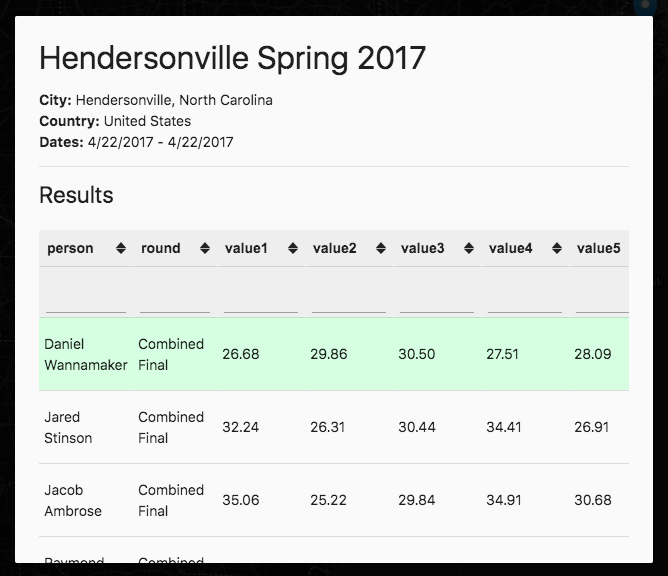
\includegraphics[scale=0.35]{competition_details.png}\\
 			\end{center}

		\subsection{Detailed Results}
			\begin{center}
				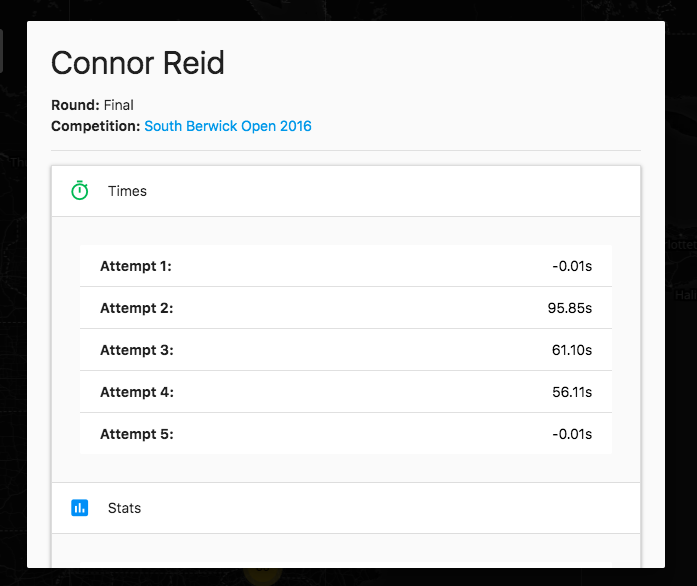
\includegraphics[scale=0.45]{result_details_times.png}\\
				\vspace{5mm}
				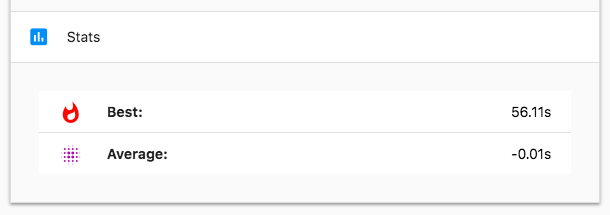
\includegraphics[scale=0.53]{result_details_stats.png}\\
 			\end{center}

		\subsection{Record Result}
			\begin{center}
				
\includegraphics[scale=0.47]{result_record.png}\\
 			\end{center}

		\subsection{Map Cluster}
			\begin{center}
				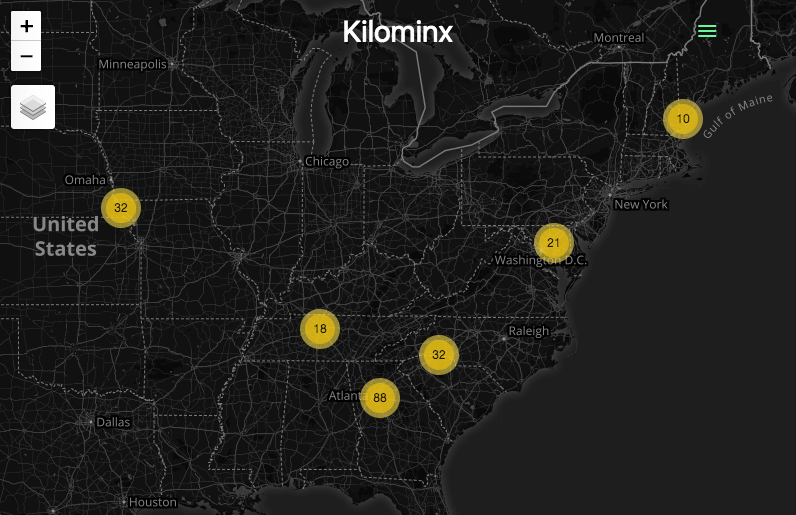
\includegraphics[scale=0.427]{map_clustering.png}\\
				\vspace{5mm}
				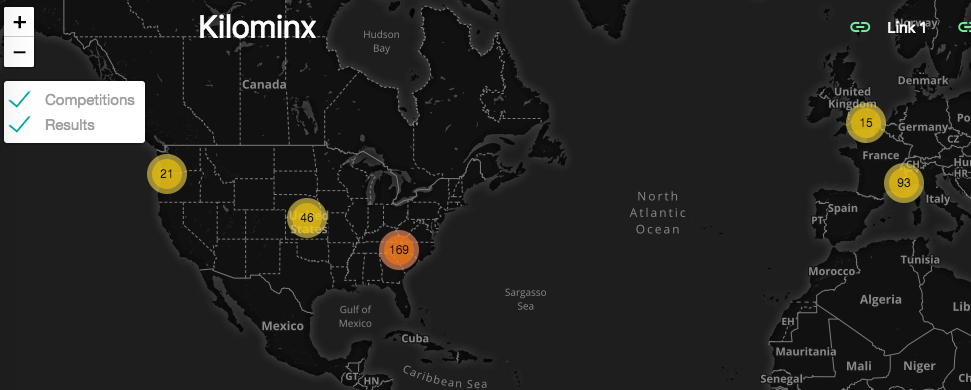
\includegraphics[scale=0.35]{map_filtering.png}\\
 			\end{center}

		\subsection{Result Marker}
			\begin{center}
				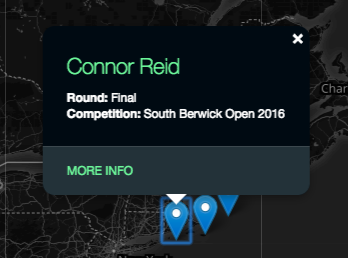
\includegraphics[scale=0.7]{result_marker.png}\\
 			\end{center}

	\section{Conclusion}
		\paragraph*{}
			Overall, I think what we created is a good foundation for an Official Kilominx Results site that could one day be trusted as a go-to resource for a more visually appealing, more easily digestible competition results in the Kilominx category of cubing than that which is available right now- a spreadsheet. A few features that could go on a "wish list" of things to be added to the application at some point in the future include the following:\\
			\tab 1) a page that conglomerates all Kilominx data for all competitions and records into 
			\tab a single, searchable, and filterable table of data, such as the one that the World Cube 
			\tab Association has on their site,\\ 
			\tab 2) a page for each registered participant that shows their results/records across all 
			\tab competitions in which they have competed, and\\ 
			\tab 3) a finished \& functioning mobile navigation interface that allows for all of the current 
			\tab and future features to be better accessed through a mobile device.

	\section{Appendix}
		\subsection{References}
			\href{https://www.worldcubeassociation.org/}{World Cube Assosiation}\\
			\href{https://ruwix.com/twisty-puzzles/kilominx/}{Kilominx}\\
			\href{https://docs.google.com/spreadsheets/d/1p8uFFILT2TkmkTodaHzeDHiWBjfqUz7YUGaOslbyR2A/edit?usp=sharing}{Official Unofficial Kilominx Result Spreadsheet}

\end{document}